После написания кода программ, необходимо было собрать робота-повора.

На рисунке 6.1 представлен манипулятор в рабочем состоянии.

\begin{figure}[h!]
\center{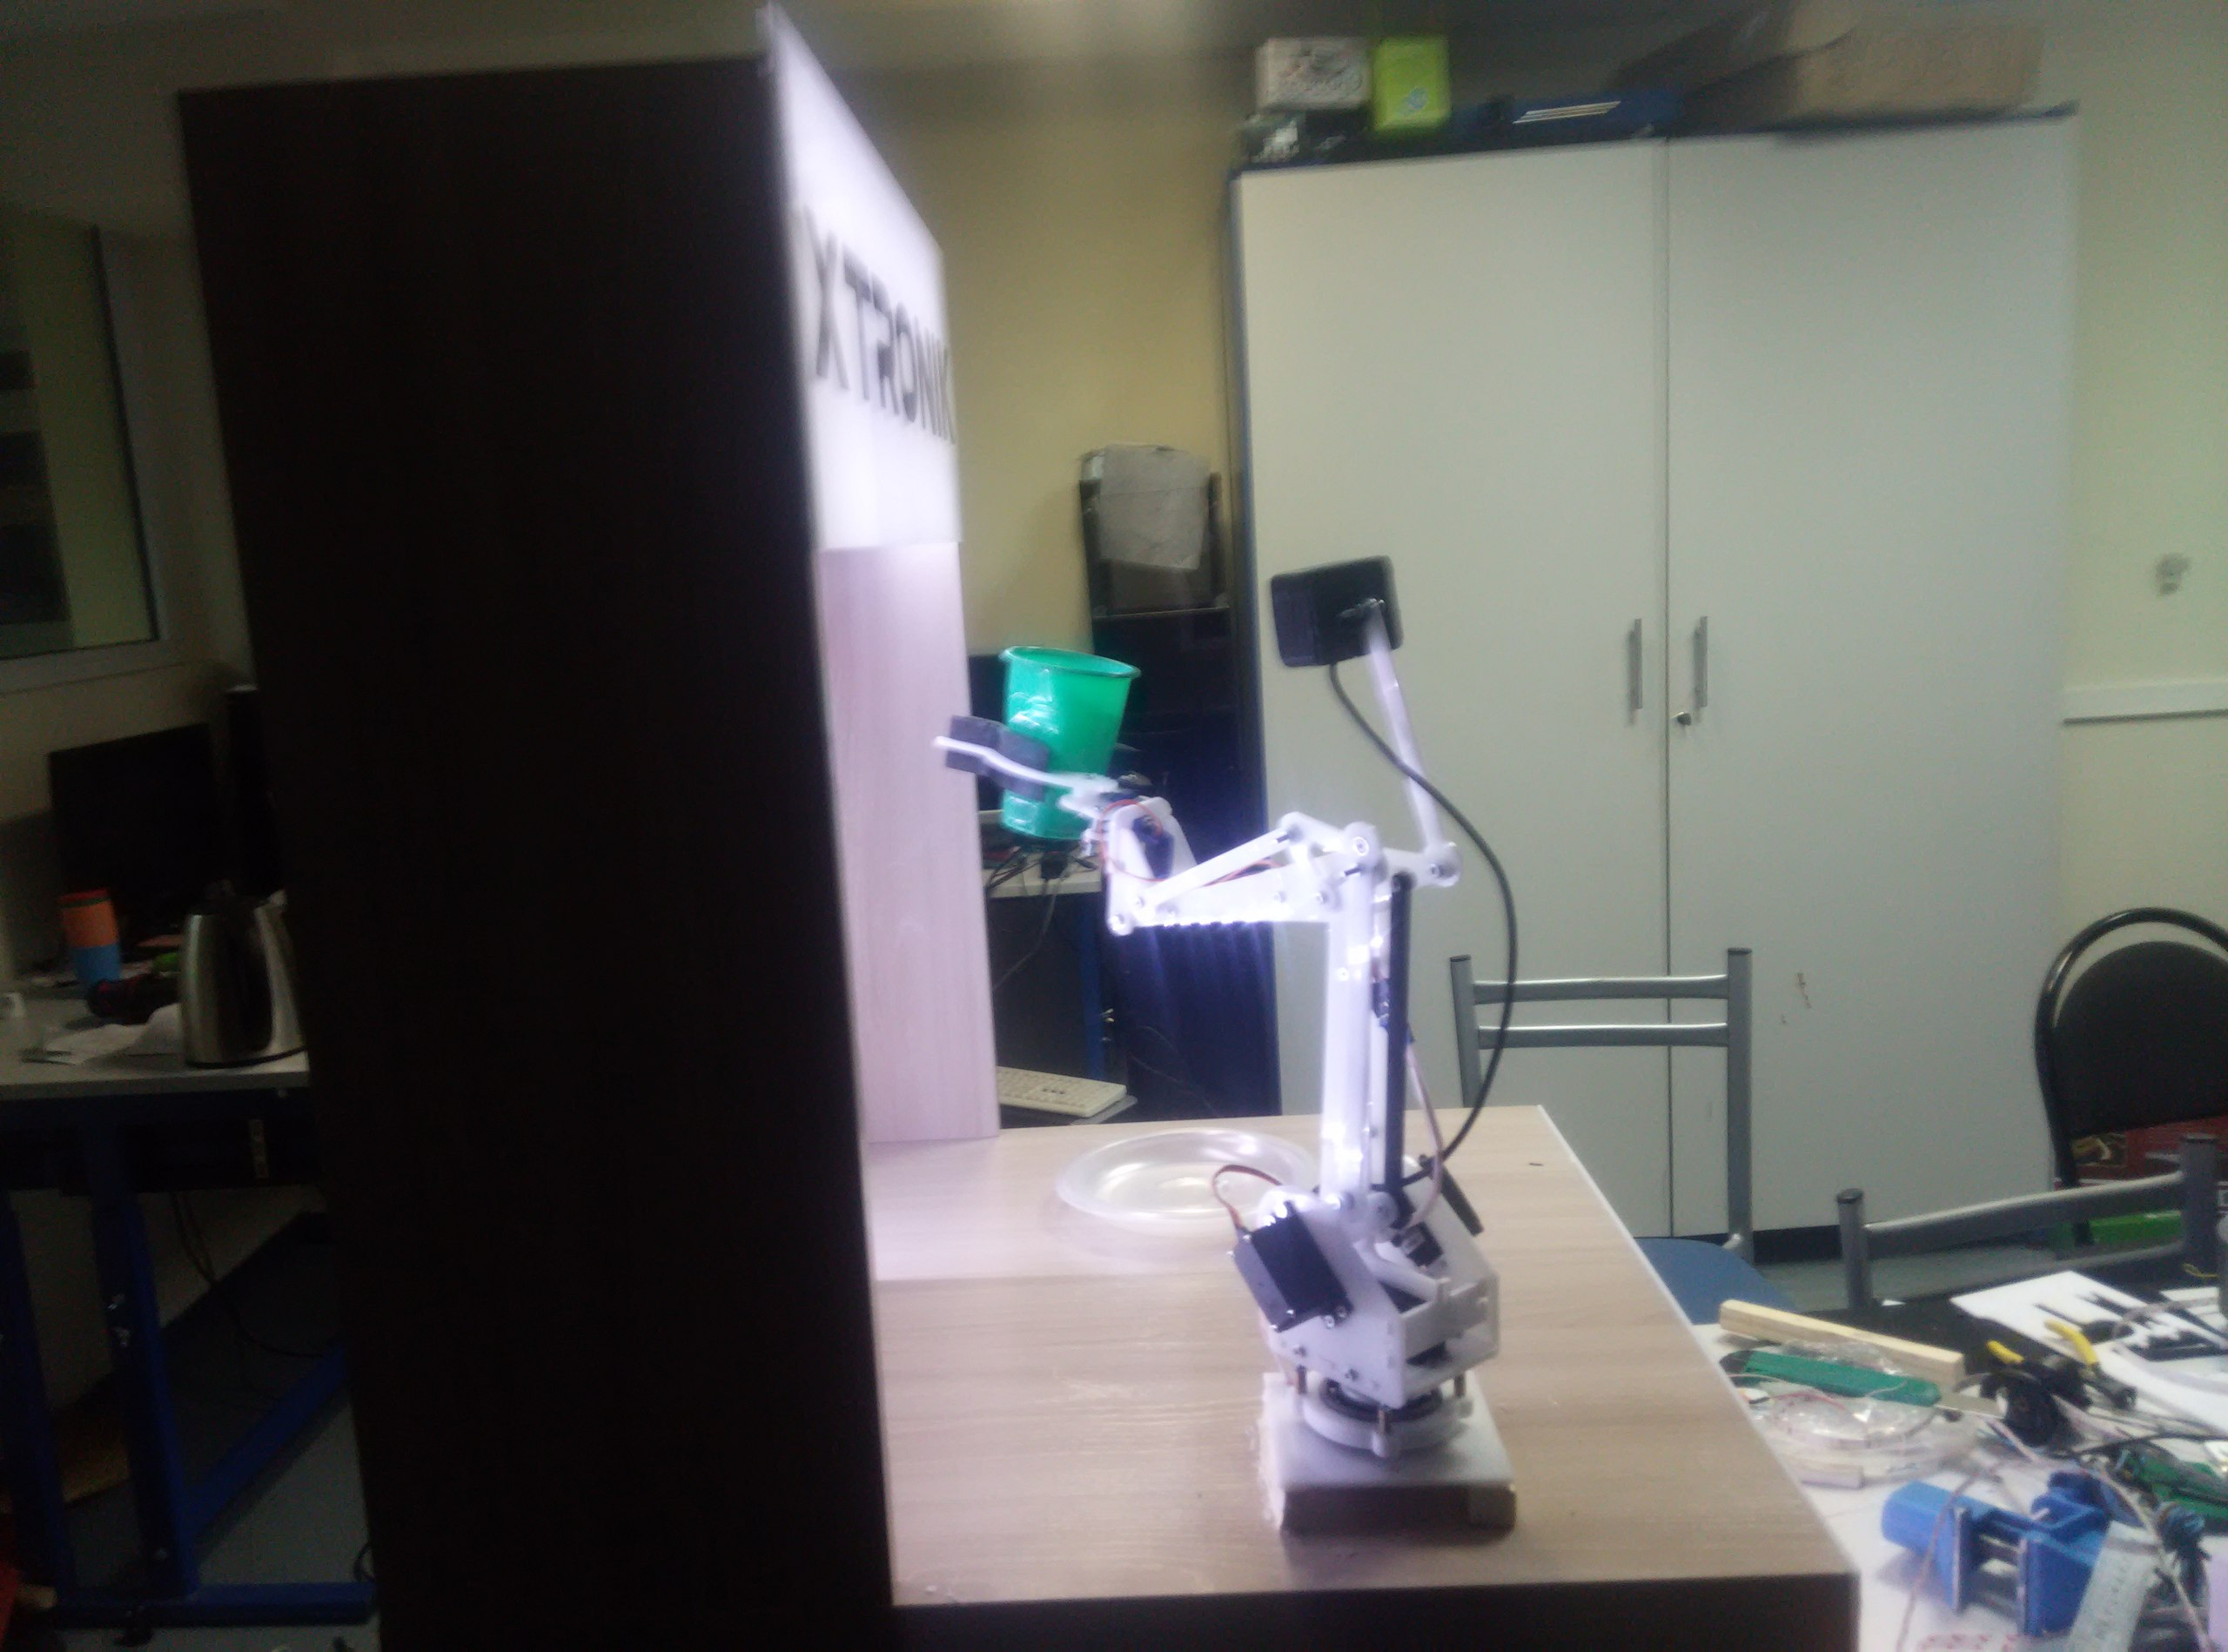
\includegraphics[width=0.85\linewidth]{images/sboku.jpg}}
\caption{Робот-повар. Вид сбоку}
\end{figure}

При испытании робота было обнаружены его недостатки:

\begin{itemize}
   	\item движения манипулятора не были плавными;
   	\item нахождение предмета сильно зависело от освещения;
   	\item захват предмета не всегда проходил успешно и в случае неудачи, манипулятор продолжал запрограммированные действия, будто предмет он захватил;
   	\item программа давала сбой и робот <<впадал в ступор>>.
\end{itemize}

Часть вышеперечисленного удалось исправить. Для улучшения процесса захвата, была поставлена более широкая <<клешня>>, а для более успешного нахождения были отредактированны параметры поиска. Сбои удалось исключить посредством улучшения качества программного кода.

Т.к. качество камеры было недостаточно высокое и сервоприводы были малой мощности, случаи незахвата предмета и ненахождения объекта остались, но были сведены к минимуму.

В финальной версии роботы выглядел, как на рисунке 6.2.

\begin{figure}[h!]
\center{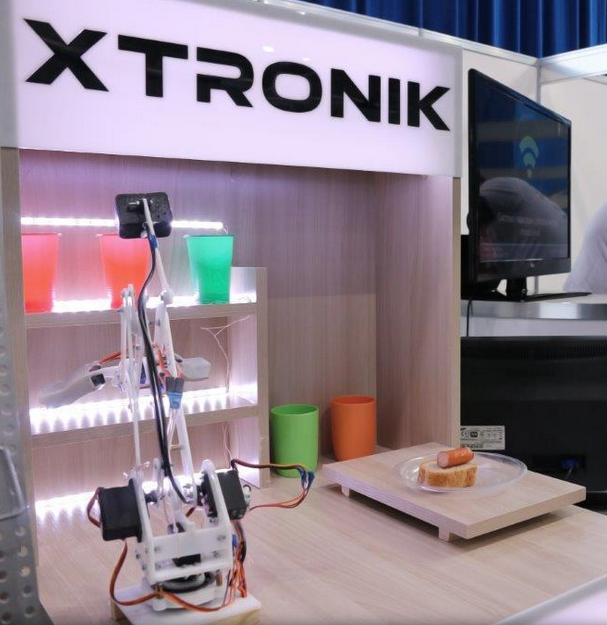
\includegraphics[width=0.85\linewidth]{images/vyst.png}}
\caption{Робот-повар в процессе сборки бутерброда}
\end{figure}

\newpage

<<Мир глазами робота>> представлен на рисунке 6.3.
 
\begin{figure}[h!]
\center{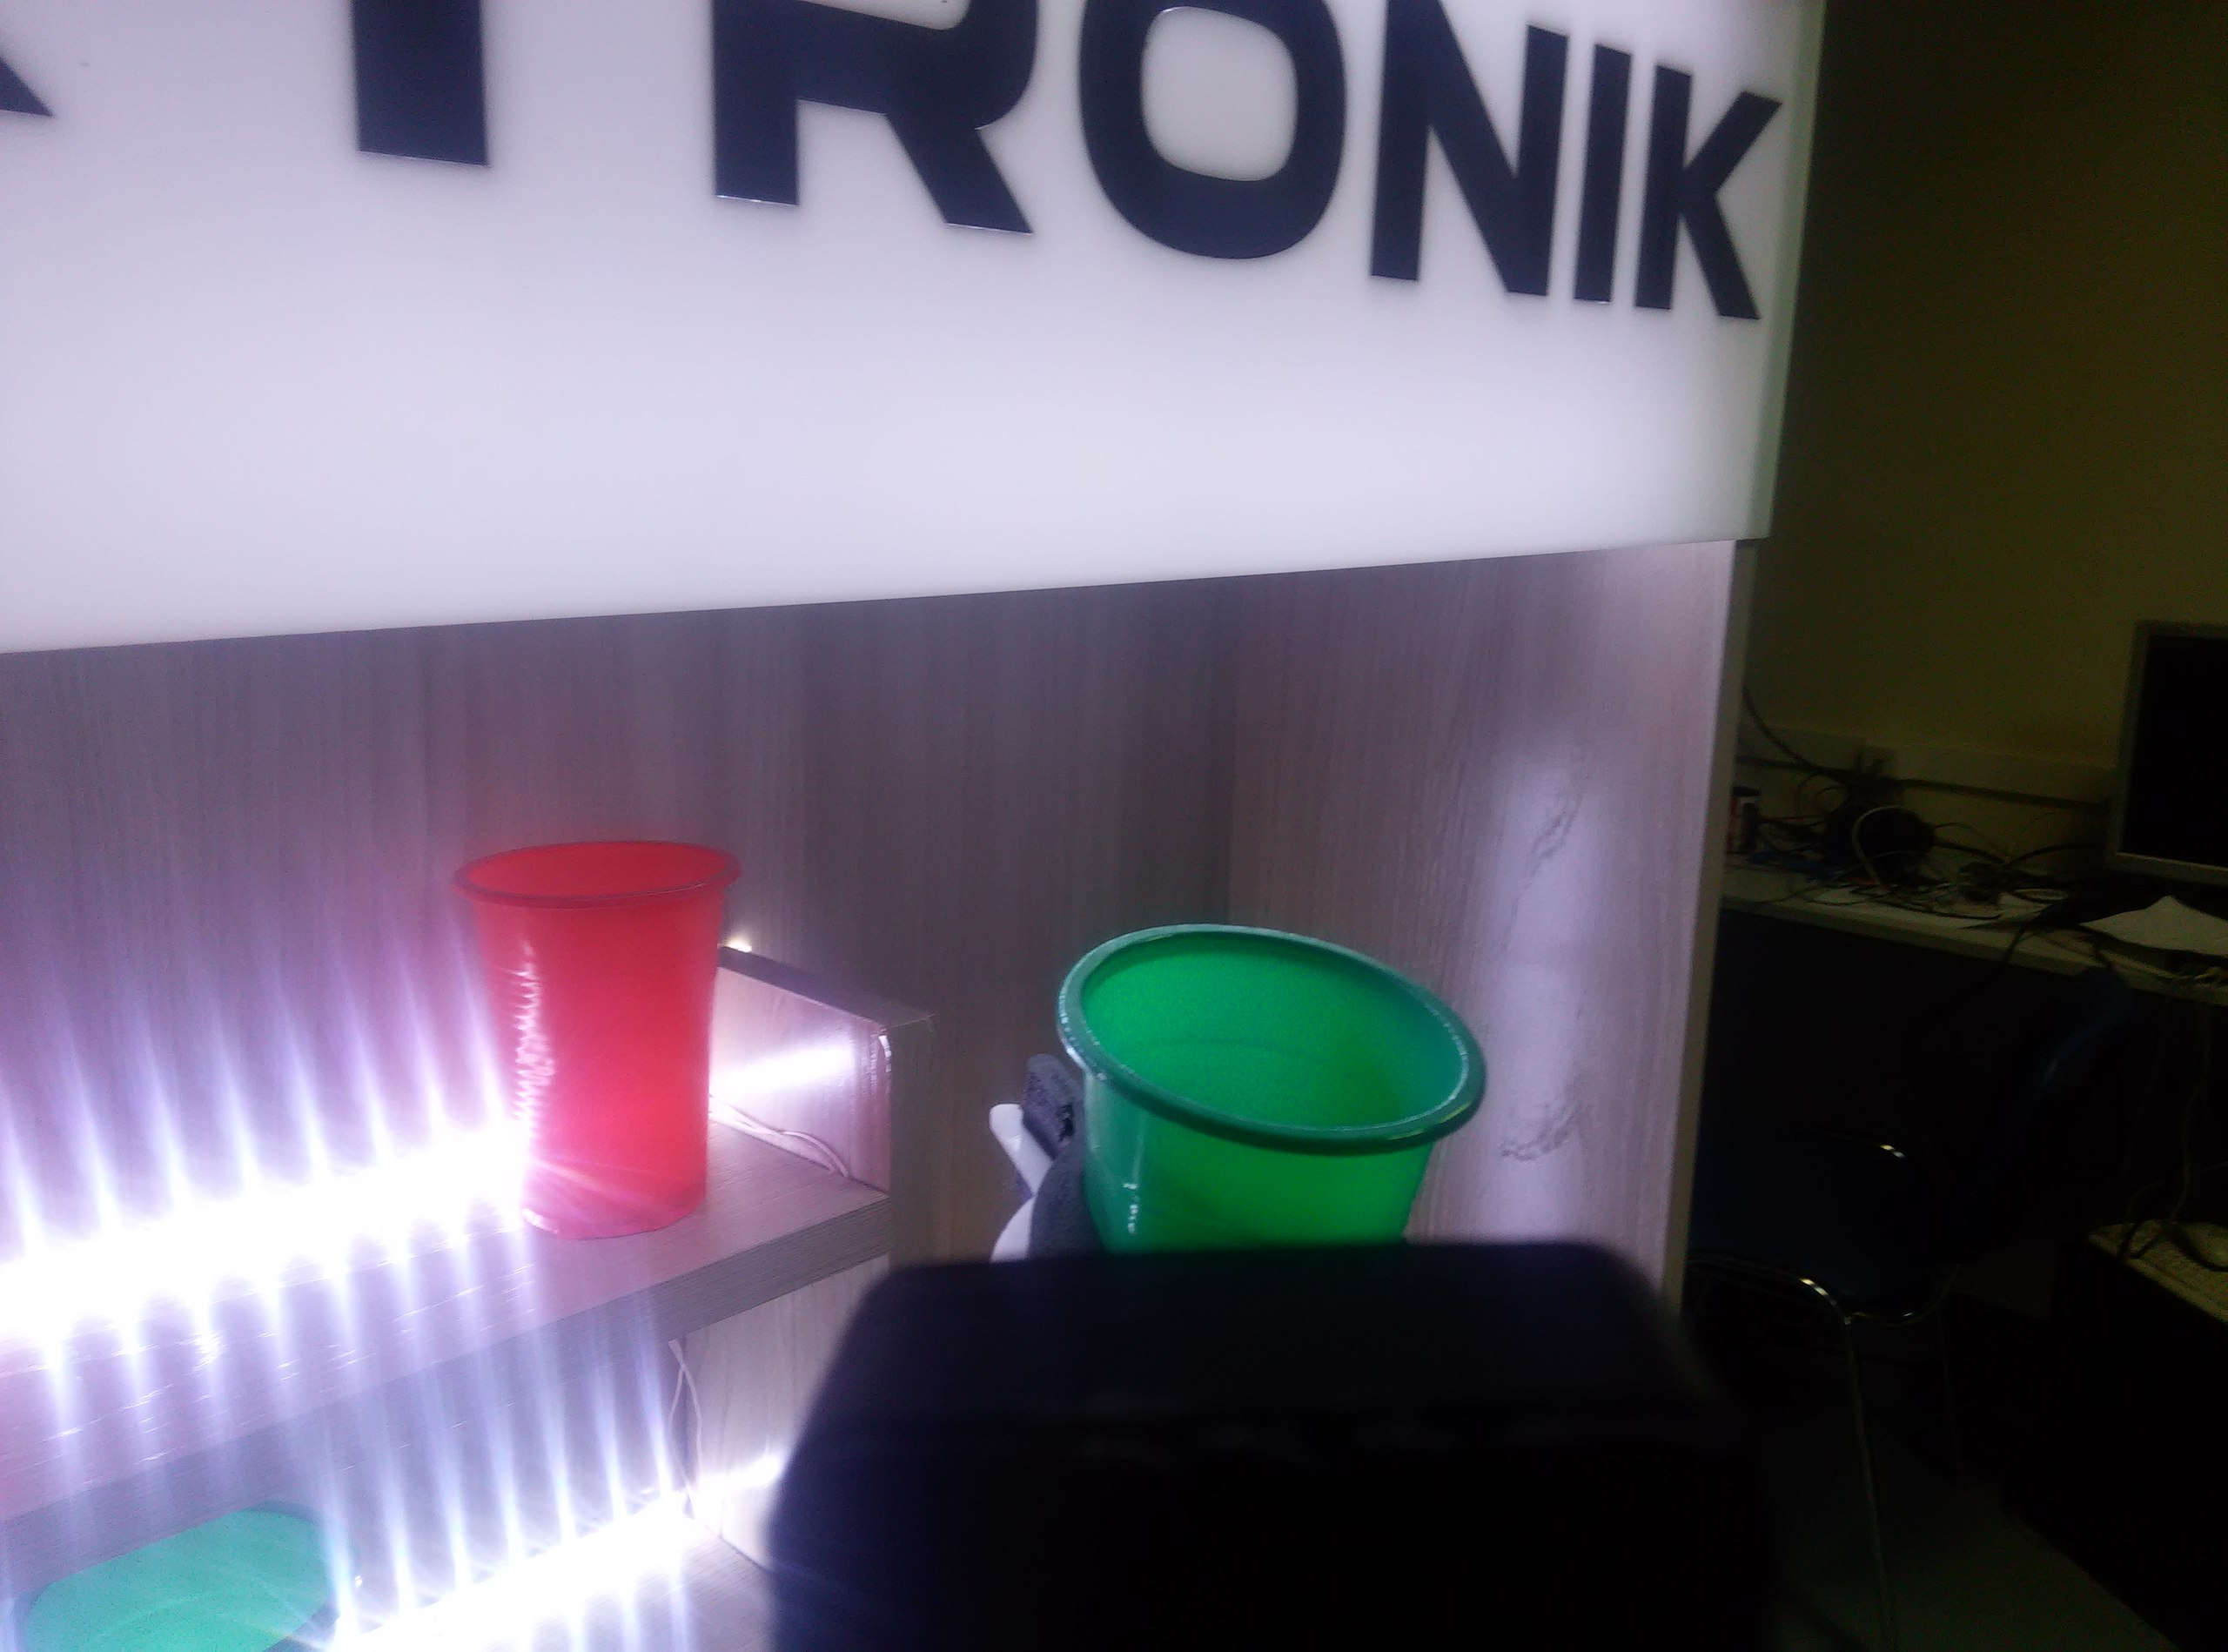
\includegraphics[width=0.85\linewidth]{images/webcam.jpg}}
\caption{Вид с вебкамеры}
\end{figure}